\documentclass[aspectratio=169]{beamer}
\usepackage[utf8]{inputenc}
\usepackage{hyperref}
\usepackage{amsmath,amsfonts,amsthm,bm}
\usepackage{color}
\usepackage{minted}
\usepackage{graphicx} % Allows including images
\usepackage{subcaption}
\usepackage{booktabs} % Allows the use of \toprule, \midrule and \bottomrule in tables
\usepackage{tikz}
%\usepackage{pgfplots}
\usepackage{listings}
\usepackage{courier}
\usepackage[version=4]{mhchem}
\usepackage{array}
\setminted{fontsize=\scriptsize}
\lstset{ %
  basicstyle=\scriptsize\ttfamily, % fonts that are used for the code
  breakatwhitespace=false,         % sets if automatic breaks should only happen at whitespace
  %breaklines=true,                 % sets automatic line breaking
  %captionpos=b,                    % sets the caption-position to bottom
  commentstyle=\color{gray}\textit,    % comment style
  keepspaces=true,                 % keeps spaces in text, useful for keeping indentation of code (possibly needs columns=flexible)
  keywordstyle=\color{blue},       % keyword style
  language=Python,                 % the language of the code
  %otherkeywords={*,...},          % if you want to add more keywords to the set
  rulecolor=\color{black},         % if not set, the frame-color may be changed on line-breaks within not-black text (e.g. comments (green here))
  showspaces=false,                % show spaces everywhere adding particular underscores; it overrides 'showstringspaces'
  showstringspaces=false,          % underline spaces within strings only
  showtabs=false,                  % show tabs within strings adding particular underscores
  stringstyle=\color{red}, % string literal style
  tabsize=4,	                   % sets default tabsize to 2 spaces
  columns=fixed                    % Using fixed column width (for e.g. nice alignment)
}

\hypersetup{
    colorlinks=true,
    linkcolor=red,
    filecolor=magenta,      
    urlcolor=red,
}

\DeclareMathOperator*{\argmax}{argmax}
\DeclareMathOperator*{\argmin}{argmin}
\let \vec \mathbf

\newcommand{\classname}{NANO266}
\newcommand{\classyear}{Fall 2024}
\mode<presentation> {
    \usetheme{CambridgeUS}
    \setbeamertemplate{footline}[text line]{%
      \parbox{\linewidth}{\vspace*{-8pt}\classname\hfill\classyear\hfill\insertpagenumber}}

    %\setbeamertemplate{footline}[page number]
    \setbeamertemplate{navigation symbols}{}
}


\title[\classname Lab 3 - Bulk properties of Crystals]{\classname~- Quantum Mechanical Modeling of Materials and Nanostructures\\Lab 3 - Bulk properties of Crystals}

\author{Shyue Ping Ong}
\institute[UCSD]{University of California, San Diego\\
\medskip
}
\date{\classyear} % Date, can be changed to a custom date

\begin{document}


\begin{frame}
    \titlepage % Print the title page as the first slide
\end{frame}


\begin{frame}{Aims of Lab 3}
\Large{
\begin{enumerate}
    \item Apply DFT to study different material properties.
\end{enumerate}
}
\end{frame}

\begin{frame}{Pressure-induced Phase Transition in Fe}
\begin{figure}
    \centering
    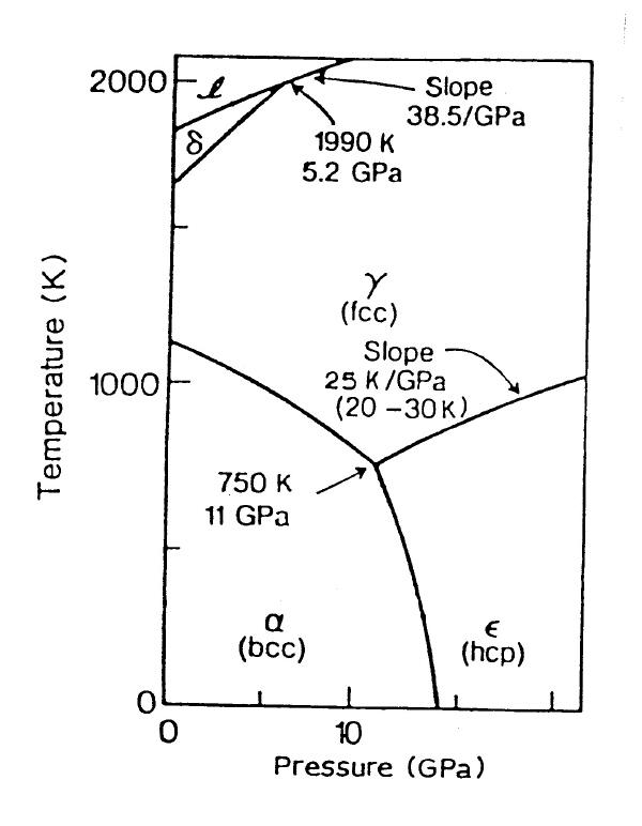
\includegraphics[width=0.4\linewidth]{lectures/figures/Lab_3-Fe_PD.png}
    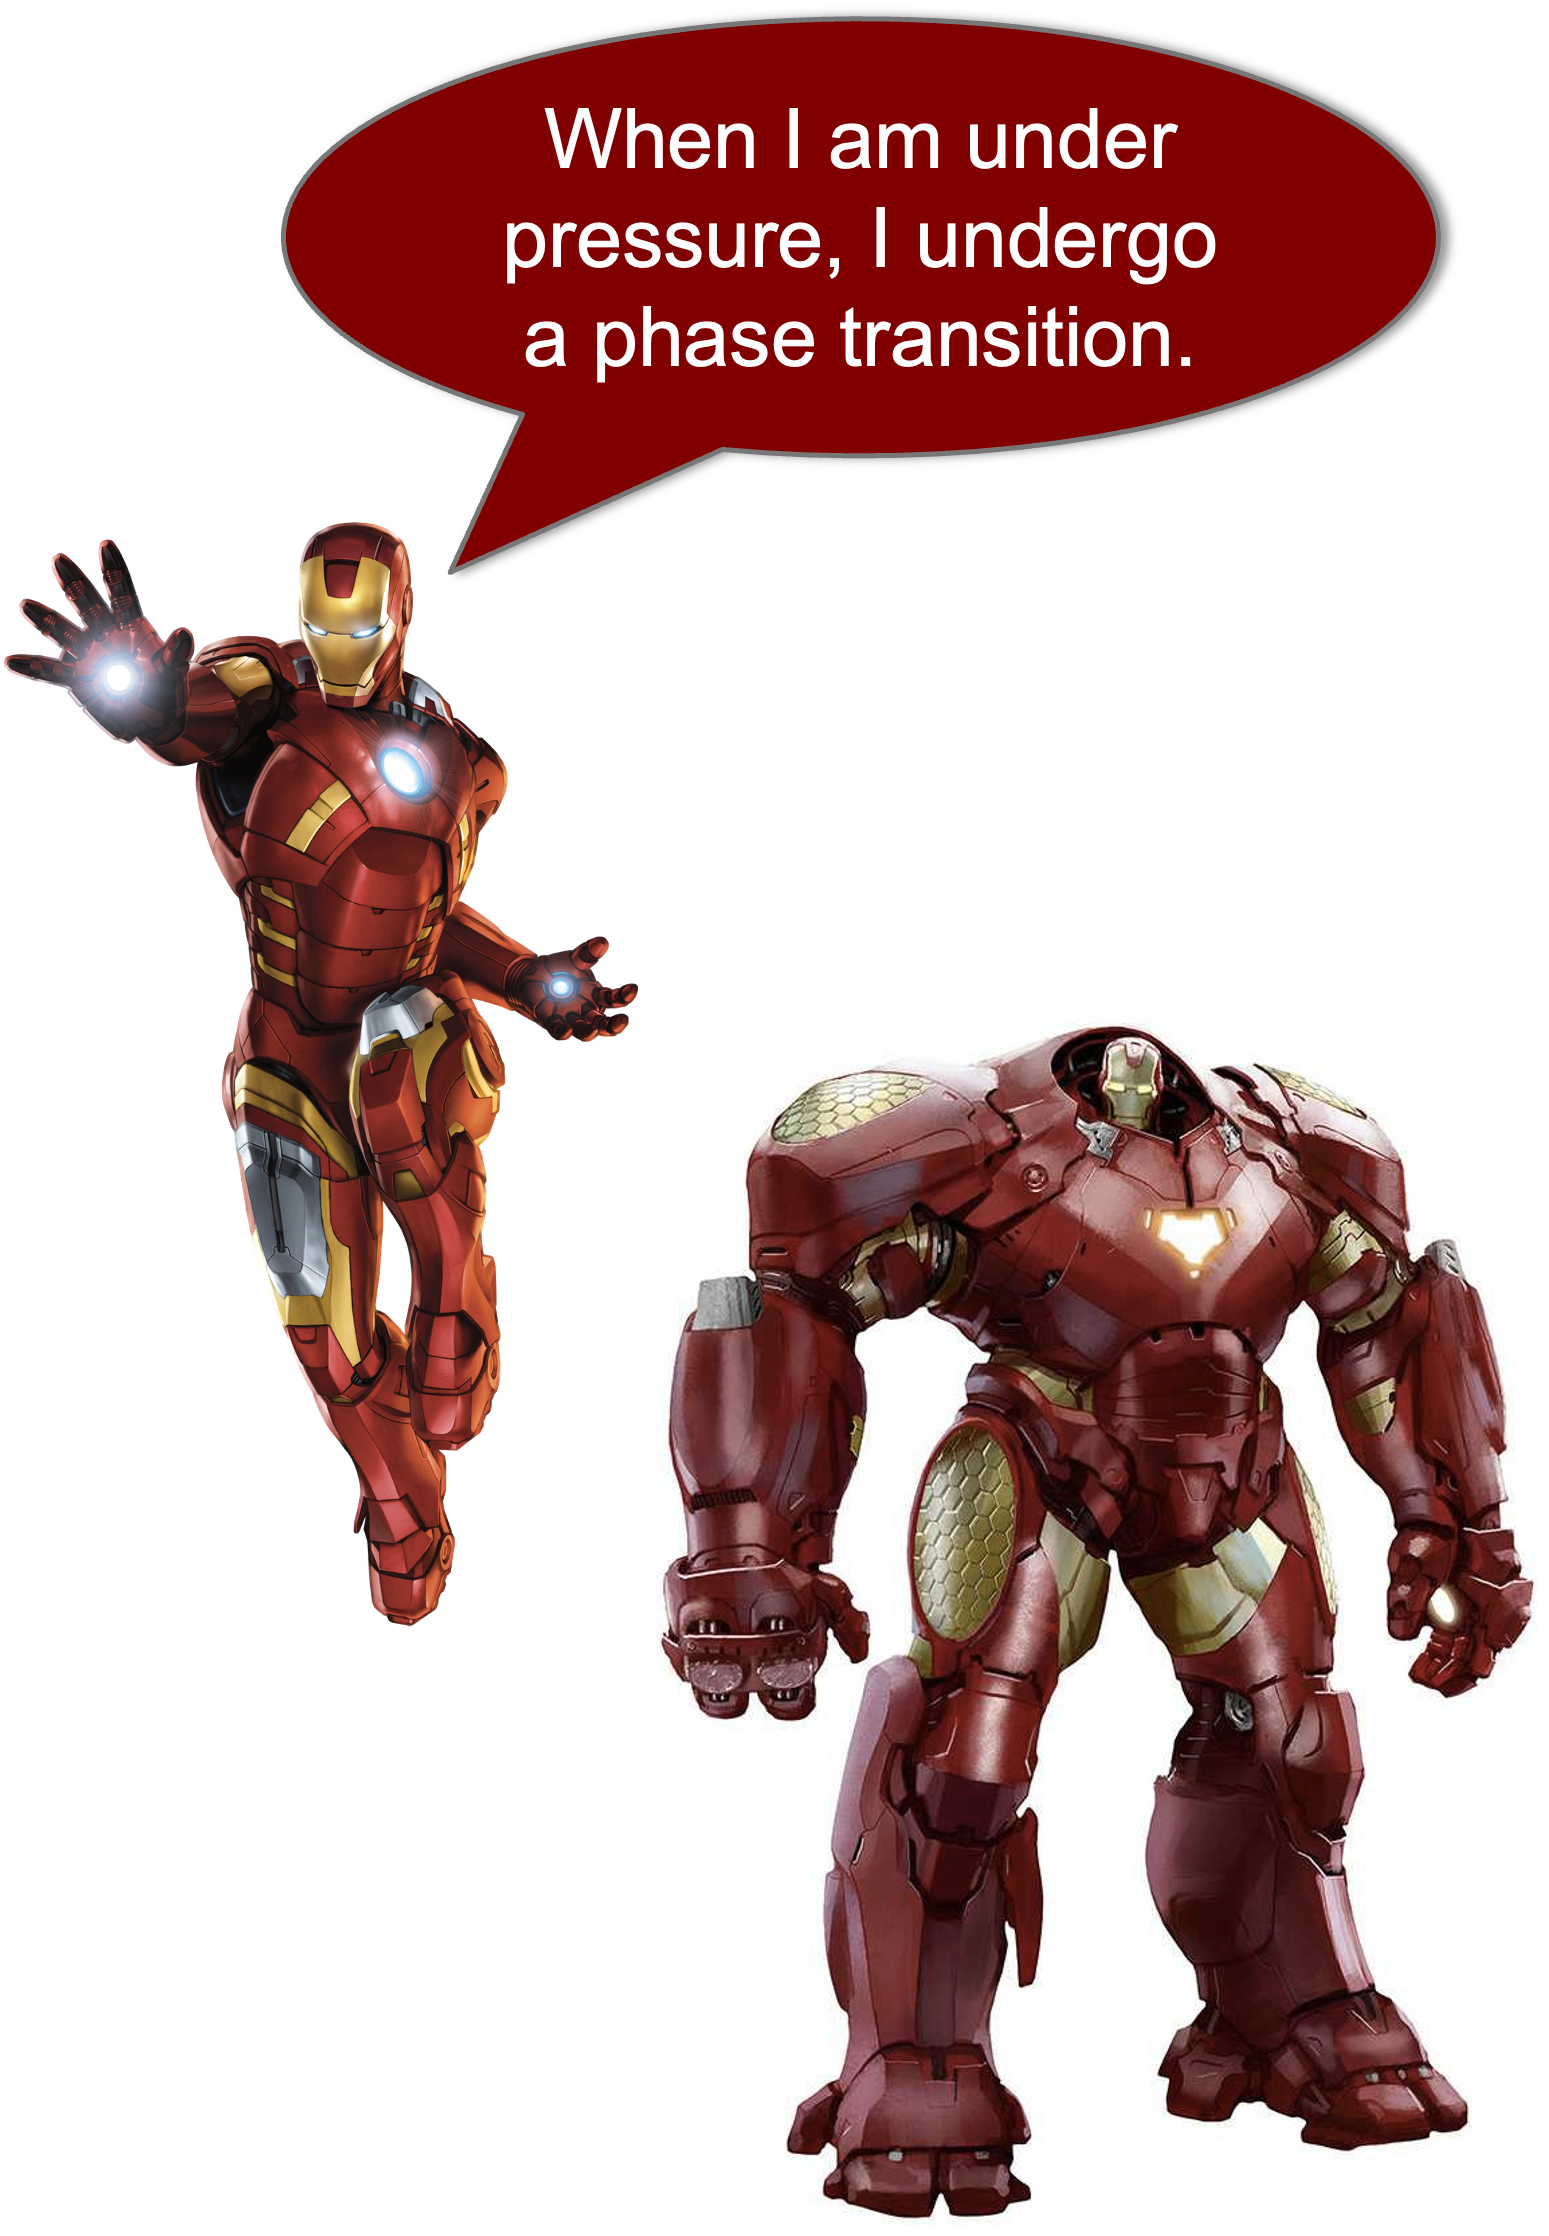
\includegraphics[width=0.3\linewidth]{lectures/figures/Lab_3-Iron_Man.png}
\end{figure} 

\end{frame} 

\begin{frame}{Symmetry Breaking in \ce{PbTiO3}}

\begin{figure}
    \centering
    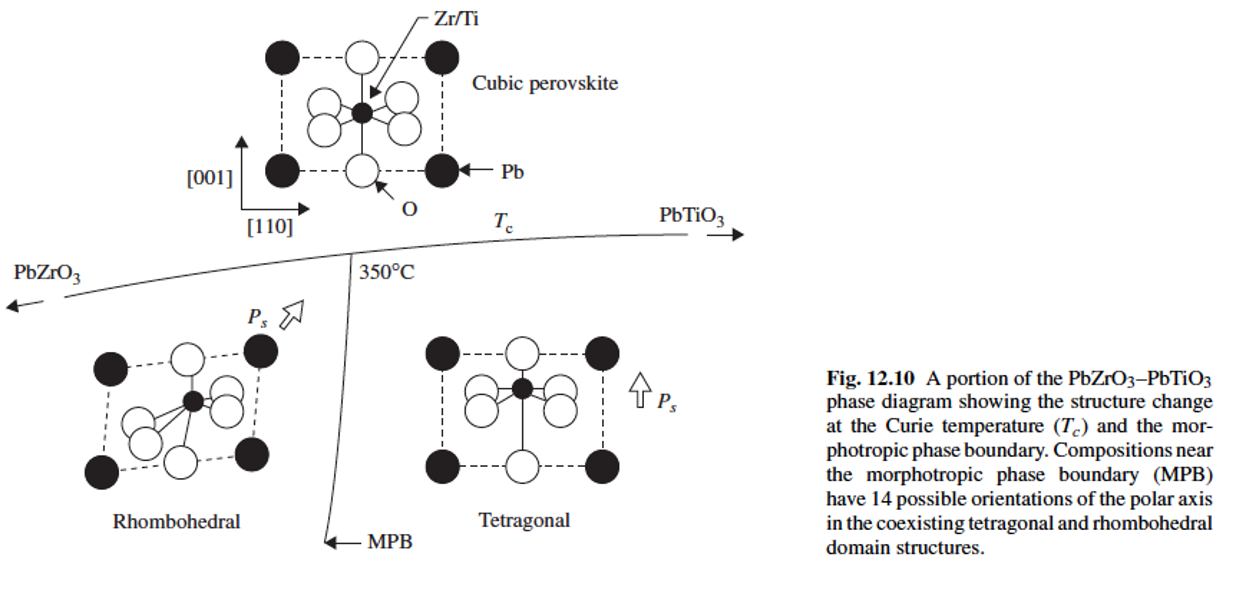
\includegraphics[width=\linewidth]{lectures/figures/Lab_3-PbTiO3.png}
\end{figure} 
\end{frame} 

\begin{frame}{Intermetallic Formation and Ordering in Cu-Au}
\begin{figure}
    \centering
    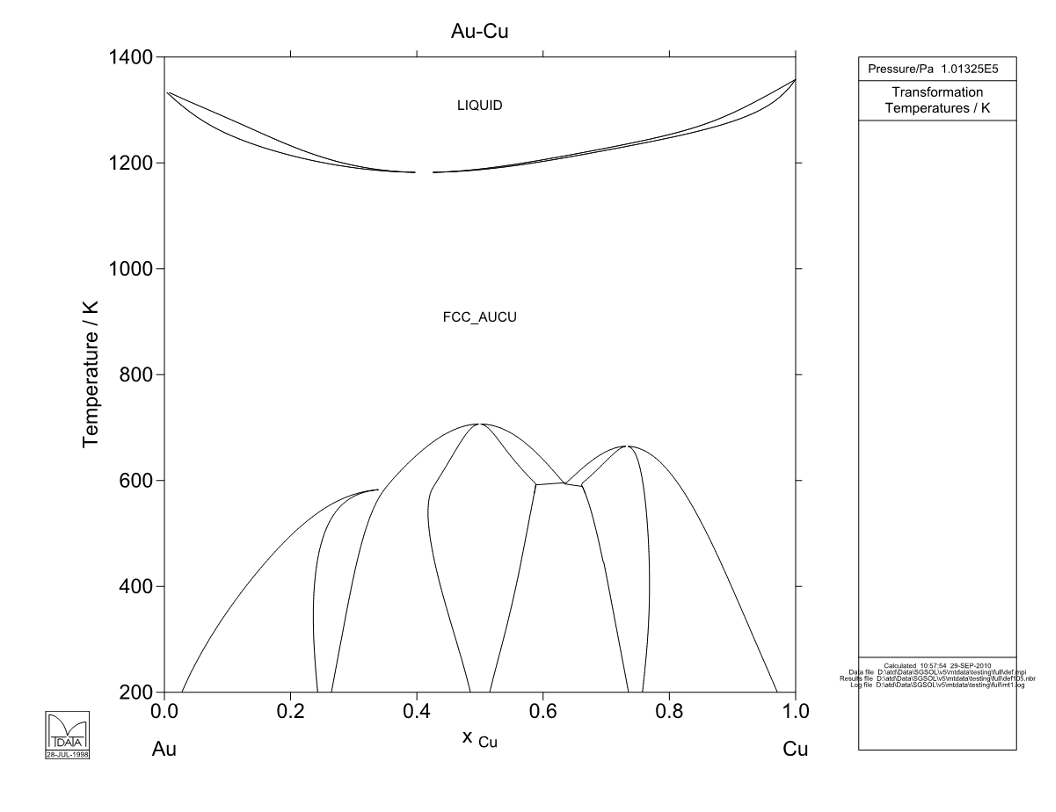
\includegraphics[width=0.6\linewidth]{lectures/figures/Lab_3-Cu_Au_PD.png}
\end{figure} 
\end{frame} 

% \begin{frame}[allowframebreaks]{Bibliography}
%     \bibliographystyle{unsrt}
%     \bibliography{refs}
% \end{frame}

\begin{frame}
    \Huge{\centerline{The End}}
\end{frame}

\end{document}

